\documentclass[11pt]{article}

\newcommand{\titrechapitre}{Suites arithmétiques et géométriques -- Cours}
\newcommand{\titreclasse}{Lycée Jean-Baptiste \textsc{Corot}}
\newcommand{\pagination}{\thepage}%/\pageref{LastPage}}
\newcommand{\topbotmargins}{2cm}
%%%%%%%%%%%%%%%%%%%%%%%%%%%%%%%%%%%%%%%%%%%%%%%%%%%%%%%%%%%%%%%%%%%%%%%%%%%%%%%%
%
% PACKAGES
% ========
%
%%%%%%%%%%%%%%%%%%%%%%%%%%%%%%%%%%%%%%%%%%%%%%%%%%%%%%%%%%%%%%%%%%%%%%%%%%%%%%%%

\usepackage[english, french]{babel}
\usepackage[utf8]{inputenc}
\usepackage[T1]{fontenc}
\usepackage{graphicx}
\usepackage{amsmath,amssymb,amsthm,amsopn}
\usepackage{hyperref}

% Pour avoir l'écriture \mathscr (math script)
% ============================================

\usepackage{mathrsfs}

% Deal with coma as a decimal separator
% =====================================

\usepackage{icomma}

% Package Geometry
% ================

\usepackage[a4paper, lmargin=2cm, rmargin=2cm, top=\topbotmargins, bottom=\topbotmargins]{geometry}

% Package multicol
% ================

\usepackage{multicol}

% Redefine abstract
% =================

% Note
% ====
%
% Le reste a été commenté pour ne pas charger trop de choses au démarrage. On
% verra si on en a besoin plus tard.
%
% --------
%
%\usepackage{mathrsfs}
%\usepackage{multirow}
%\usepackage{bm}
%\hypersetup{
%    colorlinks=true,
%    linkcolor=blue,
%    citecolor=red,
%}
%\usepackage{diagbox}
%
%\usepackage{algorithm}
%\usepackage{algpseudocode}
%
%\renewcommand{\algorithmicrequire}{\textbf{Input:}}
%\renewcommand{\algorithmicensure}{\textbf{Output:}}


%%%%%%%%%%%%%%%%%%%%%%%%%%%%%%%%%%%%%%%%%%%%%%%%%%%%%%%%%%%%%%%%%%%%%%%%%%%%%%%%
%
% TIKZ
% ====
%
%%%%%%%%%%%%%%%%%%%%%%%%%%%%%%%%%%%%%%%%%%%%%%%%%%%%%%%%%%%%%%%%%%%%%%%%%%%%%%%%

\usepackage{tikz}
\usetikzlibrary{arrows}

\usepackage{tkz-tab} % Variation tables

\usepackage{pgfplots}
%\usepackage{pgf-pie} % Pie charts

\pgfplotsset{
%\newcommand{\settingsgraph}{
x=.5cm,y=.5cm,
xticklabel style = {font=\scriptsize, yshift=.1cm},
yticklabel style = {font=\scriptsize, xshift=.1cm},
axis lines=middle,
ymajorgrids=true,
xmajorgrids=true,
major grid style = {color=white!80!blue},
xmin=-5.5,
xmax=5.5,
ymin=-5.5,
ymax=5.5,
xtick={-5.0,-4.0,...,5.0},
ytick={-5.0,-4.0,...,5.0},
}

% Tikz style

\tikzset{round/.style={circle, draw=black, very thick, scale = 0.7}}
\tikzset{arrow/.style={->, >=latex}}
\tikzset{dashed-arrow/.style={->, >=latex, dashed}}

\newcommand{\point}[3]{\draw[very thick, #3] (#1-.1, #2)--(#1+.1, #2)
(#1, #2-.1)--(#1, #2+.1)}

%%%%%%%%%%%%%%%%%%%%%%%%%%%%%%%%%%%%%%%%%%%%%%%%%%%%%%%%%%%%%%%%%%%%%%%%%%%%%%%%
%
% FANCY HEADER
% ============
%
%%%%%%%%%%%%%%%%%%%%%%%%%%%%%%%%%%%%%%%%%%%%%%%%%%%%%%%%%%%%%%%%%%%%%%%%%%%%%%%%


\usepackage{fancyhdr}
\usepackage{lastpage}

\pagestyle{fancy}
\newcommand{\changefont}{\fontsize{9}{9}\selectfont}
\renewcommand{\headrulewidth}{0mm}
\renewcommand{\footrulewidth}{0mm}

\fancyhead[C]{}
\fancyhead[L]{\titreclasse}
\fancyhead[R]{\titrechapitre}
\fancyfoot[C]{}
\fancyfoot[L]{}
\fancyfoot[R]{\pagination}
\addtolength{\skip\footins}{20pt} % distance between text and footnotes

%%%%%%%%%%%%%%%%%%%%%%%%%%%%%%%%%%%%%%%%%%%%%%%%%%%%%%%%%%%%%%%%%%%%%%%%%%%%%%%%
%
% THEOREM STYLE
% =============
%
%%%%%%%%%%%%%%%%%%%%%%%%%%%%%%%%%%%%%%%%%%%%%%%%%%%%%%%%%%%%%%%%%%%%%%%%%%%%%%%%

\usepackage[tikz]{bclogo}
\usepackage{mdframed}

\usepackage{tcolorbox}
\tcbuselibrary{listings, breakable, theorems, skins}

%\newtheoremstyle{break}%
%{}{}%
%{\itshape}{}%
%{\bfseries}{}%  % Note that final punctuation is omitted.
%{\newline}{}

\newtheoremstyle{scbf}%
{}{}%
{}{}%
%{\scshape}{}%  % Note that final punctuation is omitted.
{\bfseries\scshape}{}%  % Note that final punctuation is omitted.
{\newline}{}

%\theoremstyle{break}
%\theoremstyle{plain}
%\newtheorem{thm}{Theorem}[section]
%\newtheorem{lm}[thm]{Lemma}
%\newtheorem{prop}[thm]{Proposition}
%\newtheorem{cor}[thm]{Corollary}

%\theoremstyle{scbf}
%\newtheorem{exo}{$\star$ Exercice}

%\theoremstyle{definition}
%\newtheorem{defi}[thm]{Definition}
%\newtheorem{ex}[thm]{Example}

%\theoremstyle{remark}
%\newtheorem{rem}[thm]{Remark}

% Defining the Remark environment
% ===============================

\newenvironment{rmq}
  {
    \begin{bclogo}[logo=\bcinfo, noborder=true]{Remarque}
  }
  {
    \end{bclogo}
  }

% Defining the exercise environment
% =================================

\newcounter{exos}
\setcounter{exos}{1}

\newenvironment{exo}
  {
    \begin{bclogo}[logo=\bccrayon, noborder=true]{Exercice \theexos}
  }
  {
    \end{bclogo}
    \addtocounter{exos}{1}
  }


% Redefining the proof environment from amsthm
% ============================================

\tcolorboxenvironment{proof}{
  blanker, breakable, before skip=10pt,after skip=10pt,
  borderline west={1mm}{0pt}{red},
  left=5mm,
}

% Defining the definition environment
% ===================================

\colorlet{coldef}{black!50!green}

\newcounter{defis}
\setcounter{defis}{1}

\newenvironment{defi}[1]
  {
    \begin{defihid}{{#1}}{\thedefis}
  }
  {
    \end{defihid}
    \addtocounter{defis}{1}
  }

\newtcolorbox{defihid}[2]{%
  empty,title={ {\bfseries Définition {#2}} ({#1})},attach boxed title to top left,
boxed title style={empty,size=minimal,toprule=2pt,top=4pt,
overlay={\draw[coldef,line width=2pt]
([yshift=-1pt]frame.north west)--([yshift=-1pt]frame.north east);}},
coltitle=coldef,
before=\par\medskip\noindent,parbox=false,boxsep=0pt,left=0pt,right=3mm,top=4pt,
breakable,pad at break*=0mm,vfill before first,
overlay unbroken={\draw[coldef,line width=1pt]
([yshift=-1pt]title.north east)--([xshift=-0.5pt,yshift=-1pt]title.north-|frame.east)
--([xshift=-0.5pt]frame.south east)--(frame.south west); },
overlay first={\draw[coldef,line width=1pt]
([yshift=-1pt]title.north east)--([xshift=-0.5pt,yshift=-1pt]title.north-|frame.east)
--([xshift=-0.5pt]frame.south east); },
overlay middle={\draw[coldef,line width=1pt] ([xshift=-0.5pt]frame.north east)
--([xshift=-0.5pt]frame.south east); },
overlay last={\draw[coldef,line width=1pt] ([xshift=-0.5pt]frame.north east)
--([xshift=-0.5pt]frame.south east)--(frame.south west);},%
}

\newenvironment{notation}
  {
    \begin{notationhid}{\thedefis}
  }
  {
    \end{notationhid}
    \addtocounter{defis}{1}
  }

\newtcolorbox{notationhid}[1]{%
  empty,title={Notation {#1}},attach boxed title to top left,
boxed title style={empty,size=minimal,toprule=2pt,top=4pt,
overlay={\draw[coldef,line width=2pt]
([yshift=-1pt]frame.north west)--([yshift=-1pt]frame.north east);}},
coltitle=coldef,fonttitle=\bfseries,
before=\par\medskip\noindent,parbox=false,boxsep=0pt,left=0pt,right=3mm,top=4pt,
breakable,pad at break*=0mm,vfill before first,
overlay unbroken={\draw[coldef,line width=1pt]
([yshift=-1pt]title.north east)--([xshift=-0.5pt,yshift=-1pt]title.north-|frame.east)
--([xshift=-0.5pt]frame.south east)--(frame.south west); },
overlay first={\draw[coldef,line width=1pt]
([yshift=-1pt]title.north east)--([xshift=-0.5pt,yshift=-1pt]title.north-|frame.east)
--([xshift=-0.5pt]frame.south east); },
overlay middle={\draw[coldef,line width=1pt] ([xshift=-0.5pt]frame.north east)
--([xshift=-0.5pt]frame.south east); },
overlay last={\draw[coldef,line width=1pt] ([xshift=-0.5pt]frame.north east)
--([xshift=-0.5pt]frame.south east)--(frame.south west);},%
}


% Defining the proposition, theorem, etc. environment
% ===================================================

\colorlet{colprop}{red!75!black}

\newcounter{props}
\setcounter{props}{1}

\newenvironment{prop}
  {
    \begin{prophid}{\theprops}
  }
  {
    \end{prophid}
    \refstepcounter{props}
  }

\newtcolorbox{prophid}[1]{%
empty,title={Propriété {#1}},attach boxed title to top left,
boxed title style={empty,size=minimal,toprule=2pt,top=4pt,
overlay={\draw[colprop,line width=2pt]
([yshift=-1pt]frame.north west)--([yshift=-1pt]frame.north east);}},
coltitle=colprop,fonttitle=\bfseries,
before=\par\medskip\noindent,parbox=false,boxsep=0pt,left=0pt,right=3mm,top=4pt,
breakable,pad at break*=0mm,vfill before first,
overlay unbroken={\draw[colprop,line width=1pt]
([yshift=-1pt]title.north east)--([xshift=-0.5pt,yshift=-1pt]title.north-|frame.east)
--([xshift=-0.5pt]frame.south east)--(frame.south west); },
overlay first={\draw[colprop,line width=1pt]
([yshift=-1pt]title.north east)--([xshift=-0.5pt,yshift=-1pt]title.north-|frame.east)
--([xshift=-0.5pt]frame.south east); },
overlay middle={\draw[colprop,line width=1pt] ([xshift=-0.5pt]frame.north east)
--([xshift=-0.5pt]frame.south east); },
overlay last={\draw[colprop,line width=1pt] ([xshift=-0.5pt]frame.north east)
--([xshift=-0.5pt]frame.south east)--(frame.south west);},%
}

\newenvironment{propadm}
  {
    \begin{propadmhid}{\theprops}
  }
  {
    \end{propadmhid}
    \refstepcounter{props}
  }

  \newtcolorbox{propadmhid}[1]{%
    empty,title={{\bfseries Propriété {#1}} (admise)},attach boxed title to top left,
boxed title style={empty,size=minimal,toprule=2pt,top=4pt,
overlay={\draw[colprop,line width=2pt]
([yshift=-1pt]frame.north west)--([yshift=-1pt]frame.north east);}},
coltitle=colprop,%fonttitle=\bfseries,
before=\par\medskip\noindent,parbox=false,boxsep=0pt,left=0pt,right=3mm,top=4pt,
breakable,pad at break*=0mm,vfill before first,
overlay unbroken={\draw[colprop,line width=1pt]
([yshift=-1pt]title.north east)--([xshift=-0.5pt,yshift=-1pt]title.north-|frame.east)
--([xshift=-0.5pt]frame.south east)--(frame.south west); },
overlay first={\draw[colprop,line width=1pt]
([yshift=-1pt]title.north east)--([xshift=-0.5pt,yshift=-1pt]title.north-|frame.east)
--([xshift=-0.5pt]frame.south east); },
overlay middle={\draw[colprop,line width=1pt] ([xshift=-0.5pt]frame.north east)
--([xshift=-0.5pt]frame.south east); },
overlay last={\draw[colprop,line width=1pt] ([xshift=-0.5pt]frame.north east)
--([xshift=-0.5pt]frame.south east)--(frame.south west);},%
}

\newenvironment{propnom}[1]
  {
    \begin{propnomhid}{#1}{\theprops}
  }
  {
    \end{propnomhid}
    \refstepcounter{props}
  }

\newtcolorbox{propnomhid}[2]{%
empty,title={{\bfseries Propriété {#2}} ({#1})},attach boxed title to top left,
boxed title style={empty,size=minimal,toprule=2pt,top=4pt,
overlay={\draw[colprop,line width=2pt]
([yshift=-1pt]frame.north west)--([yshift=-1pt]frame.north east);}},
coltitle=colprop,
before=\par\medskip\noindent,parbox=false,boxsep=0pt,left=0pt,right=3mm,top=4pt,
breakable,pad at break*=0mm,vfill before first,
overlay unbroken={\draw[colprop,line width=1pt]
([yshift=-1pt]title.north east)--([xshift=-0.5pt,yshift=-1pt]title.north-|frame.east)
--([xshift=-0.5pt]frame.south east)--(frame.south west); },
overlay first={\draw[colprop,line width=1pt]
([yshift=-1pt]title.north east)--([xshift=-0.5pt,yshift=-1pt]title.north-|frame.east)
--([xshift=-0.5pt]frame.south east); },
overlay middle={\draw[colprop,line width=1pt] ([xshift=-0.5pt]frame.north east)
--([xshift=-0.5pt]frame.south east); },
overlay last={\draw[colprop,line width=1pt] ([xshift=-0.5pt]frame.north east)
--([xshift=-0.5pt]frame.south east)--(frame.south west);},%
}




\newenvironment{thm}
  {
    \begin{thmhid}{\theprops}
  }
  {
    \end{thmhid}
    \refstepcounter{props}
  }

\newtcolorbox{thmhid}[1]{%
empty,title={Théorème {#1}},attach boxed title to top left,
boxed title style={empty,size=minimal,toprule=2pt,top=4pt,
overlay={\draw[colprop,line width=2pt]
([yshift=-1pt]frame.north west)--([yshift=-1pt]frame.north east);}},
coltitle=colprop,fonttitle=\bfseries,
before=\par\medskip\noindent,parbox=false,boxsep=0pt,left=0pt,right=3mm,top=4pt,
breakable,pad at break*=0mm,vfill before first,
overlay unbroken={\draw[colprop,line width=1pt]
([yshift=-1pt]title.north east)--([xshift=-0.5pt,yshift=-1pt]title.north-|frame.east)
--([xshift=-0.5pt]frame.south east)--(frame.south west); },
overlay first={\draw[colprop,line width=1pt]
([yshift=-1pt]title.north east)--([xshift=-0.5pt,yshift=-1pt]title.north-|frame.east)
--([xshift=-0.5pt]frame.south east); },
overlay middle={\draw[colprop,line width=1pt] ([xshift=-0.5pt]frame.north east)
--([xshift=-0.5pt]frame.south east); },
overlay last={\draw[colprop,line width=1pt] ([xshift=-0.5pt]frame.north east)
--([xshift=-0.5pt]frame.south east)--(frame.south west);},%
}

\newenvironment{thmadm}
  {
    \begin{thmadmhid}{\theprops}
  }
  {
    \end{thmadmhid}
    \refstepcounter{props}
  }

  \newtcolorbox{thmadmhid}[1]{%
    empty,title={{\bfseries Théorème {#1}} (admis)},attach boxed title to top left,
boxed title style={empty,size=minimal,toprule=2pt,top=4pt,
overlay={\draw[colprop,line width=2pt]
([yshift=-1pt]frame.north west)--([yshift=-1pt]frame.north east);}},
coltitle=colprop,%fonttitle=\bfseries,
before=\par\medskip\noindent,parbox=false,boxsep=0pt,left=0pt,right=3mm,top=4pt,
breakable,pad at break*=0mm,vfill before first,
overlay unbroken={\draw[colprop,line width=1pt]
([yshift=-1pt]title.north east)--([xshift=-0.5pt,yshift=-1pt]title.north-|frame.east)
--([xshift=-0.5pt]frame.south east)--(frame.south west); },
overlay first={\draw[colprop,line width=1pt]
([yshift=-1pt]title.north east)--([xshift=-0.5pt,yshift=-1pt]title.north-|frame.east)
--([xshift=-0.5pt]frame.south east); },
overlay middle={\draw[colprop,line width=1pt] ([xshift=-0.5pt]frame.north east)
--([xshift=-0.5pt]frame.south east); },
overlay last={\draw[colprop,line width=1pt] ([xshift=-0.5pt]frame.north east)
--([xshift=-0.5pt]frame.south east)--(frame.south west);},%
}

\newenvironment{thmnom}[1]
  {
    \begin{thmnomhid}{#1}{\theprops}
  }
  {
    \end{thmnomhid}
    \refstepcounter{props}
  }

\newtcolorbox{thmnomhid}[2]{%
empty,title={{\bfseries Théorème {#2}} ({#1})},attach boxed title to top left,
boxed title style={empty,size=minimal,toprule=2pt,top=4pt,
overlay={\draw[colprop,line width=2pt]
([yshift=-1pt]frame.north west)--([yshift=-1pt]frame.north east);}},
coltitle=colprop,
before=\par\medskip\noindent,parbox=false,boxsep=0pt,left=0pt,right=3mm,top=4pt,
breakable,pad at break*=0mm,vfill before first,
overlay unbroken={\draw[colprop,line width=1pt]
([yshift=-1pt]title.north east)--([xshift=-0.5pt,yshift=-1pt]title.north-|frame.east)
--([xshift=-0.5pt]frame.south east)--(frame.south west); },
overlay first={\draw[colprop,line width=1pt]
([yshift=-1pt]title.north east)--([xshift=-0.5pt,yshift=-1pt]title.north-|frame.east)
--([xshift=-0.5pt]frame.south east); },
overlay middle={\draw[colprop,line width=1pt] ([xshift=-0.5pt]frame.north east)
--([xshift=-0.5pt]frame.south east); },
overlay last={\draw[colprop,line width=1pt] ([xshift=-0.5pt]frame.north east)
--([xshift=-0.5pt]frame.south east)--(frame.south west);},%
}

\newenvironment{coro}
  {
    \begin{corohid}{\theprops}
  }
  {
    \end{corohid}
    \refstepcounter{props}
  }

  \newtcolorbox{corohid}[1]{%
  empty,title={Corollaire {#1}},attach boxed title to top left,
boxed title style={empty,size=minimal,toprule=2pt,top=4pt,
overlay={\draw[colprop,line width=2pt]
([yshift=-1pt]frame.north west)--([yshift=-1pt]frame.north east);}},
coltitle=colprop,fonttitle=\bfseries,
before=\par\medskip\noindent,parbox=false,boxsep=0pt,left=0pt,right=3mm,top=4pt,
breakable,pad at break*=0mm,vfill before first,
overlay unbroken={\draw[colprop,line width=1pt]
([yshift=-1pt]title.north east)--([xshift=-0.5pt,yshift=-1pt]title.north-|frame.east)
--([xshift=-0.5pt]frame.south east)--(frame.south west); },
overlay first={\draw[colprop,line width=1pt]
([yshift=-1pt]title.north east)--([xshift=-0.5pt,yshift=-1pt]title.north-|frame.east)
--([xshift=-0.5pt]frame.south east); },
overlay middle={\draw[colprop,line width=1pt] ([xshift=-0.5pt]frame.north east)
--([xshift=-0.5pt]frame.south east); },
overlay last={\draw[colprop,line width=1pt] ([xshift=-0.5pt]frame.north east)
--([xshift=-0.5pt]frame.south east)--(frame.south west);},%
}

\newenvironment{lemme}
  {
    \begin{lemmehid}{\theprops}
  }
  {
    \end{lemmehid}
    \refstepcounter{props}
  }

  \newtcolorbox{lemmehid}[1]{%
  empty,title={Lemme {#1}},attach boxed title to top left,
boxed title style={empty,size=minimal,toprule=2pt,top=4pt,
overlay={\draw[colprop,line width=2pt]
([yshift=-1pt]frame.north west)--([yshift=-1pt]frame.north east);}},
coltitle=colprop,fonttitle=\bfseries,
before=\par\medskip\noindent,parbox=false,boxsep=0pt,left=0pt,right=3mm,top=4pt,
breakable,pad at break*=0mm,vfill before first,
overlay unbroken={\draw[colprop,line width=1pt]
([yshift=-1pt]title.north east)--([xshift=-0.5pt,yshift=-1pt]title.north-|frame.east)
--([xshift=-0.5pt]frame.south east)--(frame.south west); },
overlay first={\draw[colprop,line width=1pt]
([yshift=-1pt]title.north east)--([xshift=-0.5pt,yshift=-1pt]title.north-|frame.east)
--([xshift=-0.5pt]frame.south east); },
overlay middle={\draw[colprop,line width=1pt] ([xshift=-0.5pt]frame.north east)
--([xshift=-0.5pt]frame.south east); },
overlay last={\draw[colprop,line width=1pt] ([xshift=-0.5pt]frame.north east)
--([xshift=-0.5pt]frame.south east)--(frame.south west);},%
}

\colorlet{colexemple}{blue!50!black}
%\newtcolorbox{exemple}{empty, title=Exemple, attach boxed title to top left,
%  boxed title style={empty, size=minimal, toprule=2pt, top=4pt,
%    overlay={\draw[colexemple,line width=2pt]
%([yshift=-1pt]frame.north west)--([yshift=-1pt]frame.north east);}},
%coltitle=colexemple,fonttitle=\bfseries,%\large\bfseries,
%before=\par\medskip\noindent,parbox=false,boxsep=0pt,left=0pt,right=3mm,top=4pt,
%overlay={\draw[colexemple,line width=1pt]
%([yshift=-1pt]title.north east)--([xshift=-0.5pt,yshift=-1pt]title.north-|frame.east)
%--([xshift=-0.5pt]frame.south east)--(frame.south west); },
%}

\newcounter{exemples}
\setcounter{exemples}{1}

\newenvironment{exemple}
  {
    \begin{exemplehid}{\theexemples}
  }
  {
    \end{exemplehid}
    \addtocounter{exemples}{1}
  }

\newtcolorbox{exemplehid}[1]{%
empty,title={Exemple {#1}},attach boxed title to top left,
boxed title style={empty,size=minimal,toprule=2pt,top=4pt,
overlay={\draw[colexemple,line width=2pt]
([yshift=-1pt]frame.north west)--([yshift=-1pt]frame.north east);}},
coltitle=colexemple,fonttitle=\bfseries,
before=\par\medskip\noindent,parbox=false,boxsep=0pt,left=0pt,right=3mm,top=4pt,
breakable,pad at break*=0mm,vfill before first,
overlay unbroken={\draw[colexemple,line width=1pt]
([yshift=-1pt]title.north east)--([xshift=-0.5pt,yshift=-1pt]title.north-|frame.east)
--([xshift=-0.5pt]frame.south east)--(frame.south west); },
overlay first={\draw[colexemple,line width=1pt]
([yshift=-1pt]title.north east)--([xshift=-0.5pt,yshift=-1pt]title.north-|frame.east)
--([xshift=-0.5pt]frame.south east); },
overlay middle={\draw[colexemple,line width=1pt] ([xshift=-0.5pt]frame.north east)
--([xshift=-0.5pt]frame.south east); },
overlay last={\draw[colexemple,line width=1pt] ([xshift=-0.5pt]frame.north east)
--([xshift=-0.5pt]frame.south east)--(frame.south west);},%
}

\newenvironment{contrex}
  {
    \begin{contrexhid}{\theexemples}
  }
  {
    \end{contrexhid}
    \addtocounter{exemples}{1}
  }

\newtcolorbox{contrexhid}[1]{%
empty,title={Contre-exemple {#1}},attach boxed title to top left,
boxed title style={empty,size=minimal,toprule=2pt,top=4pt,
overlay={\draw[colexemple,line width=2pt]
([yshift=-1pt]frame.north west)--([yshift=-1pt]frame.north east);}},
coltitle=colexemple,fonttitle=\bfseries,
before=\par\medskip\noindent,parbox=false,boxsep=0pt,left=0pt,right=3mm,top=4pt,
breakable,pad at break*=0mm,vfill before first,
overlay unbroken={\draw[colexemple,line width=1pt]
([yshift=-1pt]title.north east)--([xshift=-0.5pt,yshift=-1pt]title.north-|frame.east)
--([xshift=-0.5pt]frame.south east)--(frame.south west); },
overlay first={\draw[colexemple,line width=1pt]
([yshift=-1pt]title.north east)--([xshift=-0.5pt,yshift=-1pt]title.north-|frame.east)
--([xshift=-0.5pt]frame.south east); },
overlay middle={\draw[colexemple,line width=1pt] ([xshift=-0.5pt]frame.north east)
--([xshift=-0.5pt]frame.south east); },
overlay last={\draw[colexemple,line width=1pt] ([xshift=-0.5pt]frame.north east)
--([xshift=-0.5pt]frame.south east)--(frame.south west);},%
}

\newenvironment{app}
  {
    \begin{apphid}{\theexemples}
  }
  {
    \end{apphid}
    \addtocounter{exemples}{1}
  }

\newtcolorbox{apphid}[1]{%
empty,title={Application {#1}},attach boxed title to top left,
boxed title style={empty,size=minimal,toprule=2pt,top=4pt,
overlay={\draw[colexemple,line width=2pt]
([yshift=-1pt]frame.north west)--([yshift=-1pt]frame.north east);}},
coltitle=colexemple,fonttitle=\bfseries,
before=\par\medskip\noindent,parbox=false,boxsep=0pt,left=0pt,right=3mm,top=4pt,
breakable,pad at break*=0mm,vfill before first,
overlay unbroken={\draw[colexemple,line width=1pt]
([yshift=-1pt]title.north east)--([xshift=-0.5pt,yshift=-1pt]title.north-|frame.east)
--([xshift=-0.5pt]frame.south east)--(frame.south west); },
overlay first={\draw[colexemple,line width=1pt]
([yshift=-1pt]title.north east)--([xshift=-0.5pt,yshift=-1pt]title.north-|frame.east)
--([xshift=-0.5pt]frame.south east); },
overlay middle={\draw[colexemple,line width=1pt] ([xshift=-0.5pt]frame.north east)
--([xshift=-0.5pt]frame.south east); },
overlay last={\draw[colexemple,line width=1pt] ([xshift=-0.5pt]frame.north east)
--([xshift=-0.5pt]frame.south east)--(frame.south west);},%
}

%%%%%%%%%%%%%%%%%%%%%%%%%%%%%%%%%%%%%%%%%%%%%%%%%%%%%%%%%%%%%%%%%%%%%%%%%%%%%%%%
%
% ENUMERATE
% =========
%
%%%%%%%%%%%%%%%%%%%%%%%%%%%%%%%%%%%%%%%%%%%%%%%%%%%%%%%%%%%%%%%%%%%%%%%%%%%%%%%%

\usepackage{enumerate}
\usepackage{enumitem}

% To have special enumerate items like
%
% 1/
% 2/
% 3/

%%%%%%%%%%%%%%%%%%%%%%%%%%%%%%%%%%%%%%%%%%%%%%%%%%%%%%%%%%%%%%%%%%%%%%%%%%%%%%%%
%
% ARRAYS
% ======
%
%%%%%%%%%%%%%%%%%%%%%%%%%%%%%%%%%%%%%%%%%%%%%%%%%%%%%%%%%%%%%%%%%%%%%%%%%%%%%%%%


\usepackage{array}
\usepackage{makecell} % Used to break lines within arrays
\usepackage{multirow}
\usepackage{booktabs} % Used to have nice arrays with headrules

%%%%%%%%%%%%%%%%%%%%%%%%%%%%%%%%%%%%%%%%%%%%%%%%%%%%%%%%%%%%%%%%%%%%%%%%%%%%%%%%
%
% WRITE CODE
% ==========
%
%%%%%%%%%%%%%%%%%%%%%%%%%%%%%%%%%%%%%%%%%%%%%%%%%%%%%%%%%%%%%%%%%%%%%%%%%%%%%%%%

\usepackage{listings}
\usepackage{xcolor}

%New colors defined below
\definecolor{codegreen}{rgb}{0,0.6,0}
\definecolor{codegray}{rgb}{0.5,0.5,0.5}
\definecolor{codepurple}{rgb}{0.58,0,0.82}
\definecolor{backcolour}{rgb}{0.95,0.95,0.92}

%Code listing style named "mystyle"
\lstdefinestyle{python}{
  %backgroundcolor=\color{backcolour},
  commentstyle=\color{codegreen},
  keywordstyle=\color{magenta},
  numberstyle=\tiny\color{codegray},
  stringstyle=\color{codepurple},
  basicstyle=\ttfamily\footnotesize,
  breakatwhitespace=false,
  breaklines=true,
  captionpos=b,
  keepspaces=true,
  numbers=left,
  numbersep=5pt,
  showspaces=false,
  showstringspaces=false,
  showtabs=false,
  tabsize=2
}

\lstset{style=python}

%%%%%%%%%%%%%%%%%%%%%%%%%%%%%%%%%%%%%%%%%%%%%%%%%%%%%%%%%%%%%%%%%%%%%%%%%%%%%%%%
%
% Tabular 
% =======
%
%%%%%%%%%%%%%%%%%%%%%%%%%%%%%%%%%%%%%%%%%%%%%%%%%%%%%%%%%%%%%%%%%%%%%%%%%%%%%%%%

% In order to obtain a tabular with given width.

\usepackage{tabularx}
\newcolumntype{Y}{>{\centering\arraybackslash}X}
\newcolumntype{R}{>{\raggedright\arraybackslash}X}
\newcolumntype{L}{>{\raggedleft\arraybackslash}X}
% \usepackage{tabulary} % younger brother

%%%%%%%%%%%%%%%%%%%%%%%%%%%%%%%%%%%%%%%%%%%%%%%%%%%%%%%%%%%%%%%%%%%%%%%%%%%%%%%%
%
% MACROS
% ======
%
%%%%%%%%%%%%%%%%%%%%%%%%%%%%%%%%%%%%%%%%%%%%%%%%%%%%%%%%%%%%%%%%%%%%%%%%%%%%%%%%

% Math Operators

\DeclareMathOperator{\Card}{Card}
\DeclareMathOperator{\Gal}{Gal}
\DeclareMathOperator{\Id}{Id}
\DeclareMathOperator{\Img}{Im}
\DeclareMathOperator{\Ker}{Ker}
\DeclareMathOperator{\Minpoly}{Minpoly}
\DeclareMathOperator{\Mod}{mod}
\DeclareMathOperator{\Ord}{Ord}
\DeclareMathOperator{\ppcm}{ppcm}
\DeclareMathOperator{\pgcd}{pgcd}
\DeclareMathOperator{\tr}{Tr}
\DeclareMathOperator{\Vect}{Vect}
\DeclareMathOperator{\Span}{Span}
\DeclareMathOperator{\rank}{rank}
\DeclareMathOperator{\rg}{rg}
\DeclareMathOperator{\ev}{ev}
\DeclareMathOperator{\Var}{Var}

% Shortcuts

\newcommand{\eg}{\emph{e.g. }}
\newcommand{\ent}[2]{[\![#1,#2]\!]}
\newcommand{\ie}{\emph{i.e. }}
\newcommand{\ps}[2]{\left\langle#1,#2\right\rangle}
\newcommand{\eqdef}{\overset{\text{def}}{=}}
\newcommand{\E}{\mathcal{E}}
\newcommand{\M}{\mathcal{M}}
\newcommand{\A}{\mathcal{A}}
\newcommand{\B}{\mathcal{B}}
\newcommand{\R}{\mathcal{R}}
\newcommand{\D}{\mathcal{D}}
\newcommand{\Pcal}{\mathcal{P}}
\newcommand{\K}{\mathbf{k}}
\newcommand{\vect}[1]{\overrightarrow{#1}}


%\input{layout-nb.tex}

\title{Chapitre 9 : Suites arithmétiques et géométriques}
\date{}
\author{}

% Note
% ====
%
% Ce chapitre doit probablement commencer par une activité pour que la
% définition de variable aléatoire soit motivée directement. Sans cela, le
% début du chapitre peut paraître un peu rude.

\begin{document}
\maketitle\thispagestyle{fancy}

\section{Suites arithmétiques}
\subsection{Définition}
\begin{defi}{Suite arithmétique}
  On dit que la suite $(u_n)$ est \textbf{arithmétique} s'il existe un réel
  $r$ tel que, pour tout entier $n\in\mathbb{N}$
  \[
    u_{n+1} = u_n + r.
  \]
  Le nombre $r$ est appelé la \textbf{raison} de la suite.

  \begin{center}
    \begin{tikzpicture}
      \node[circle, draw, minimum size=12mm] (u0) at (0,0) {$u_0$};
      \node[circle, draw, minimum size=12mm] (u1) at (3,0) {$u_1$};
      \node[circle, draw, minimum size=12mm] (u2) at (6,0) {$u_2$};
      \node[circle, draw, minimum size=12mm] (un) at (9,0) {$u_n$};
      \node[circle, draw, minimum size=12mm] (un+1) at (12,0) {$u_{n+1}$};
      \draw[-latex] (u0.north) to[out=60, in=120] (u1.north);
      \draw[-latex] (u1.north) to[out=60, in=120] (u2.north);
      \draw[-latex] (un.north) to[out=60, in=120] (un+1.north);
      \node at (1.5, .8) {$+r$};
      \node at (4.5, .8) {$+r$};
      \node at (10.5, .8) {$+r$};
      \node at (7.5,0) {$\dots$};
      \node at (13.5,0) {$\dots$};
    \end{tikzpicture}
  \end{center}
\end{defi}

\begin{rmq}
  \begin{itemize}
    \item Pour passer d'un terme à l'autre, on ajoute la raison $r$, on a donc
      $\forall n\in\mathbb{N},\;r=u_{n+1}-u_n$.
    \item La raison $r$ ne dépend pas de $n$.
  \end{itemize}
\end{rmq}

\begin{app}
  Pour chacune des suites suivantes, déterminer si elles sont arithmétiques ou
  non. Si oui, déterminer la raison et le premier terme.
  \begin{enumerate}
    \item La suite $(a_n)$ définie sur $\mathbb{N}$ par $a_0=1$ et
      $a_{n+1}=a_n-8$.
    \item La suite $(b_n)$ définie sur $\mathbb{N}$ par $b_n=n^2+2n+4$.
    \item La suite $(c_n)$ définie sur $\mathbb{N}$ par $c_n=3n+1$.
  \end{enumerate}
\end{app}

\subsection{Expression}
\begin{prop}
  Soit $(u_n)$ une suite arithmétique de raison $r$ et de premier terme $u_0$.
  Pour tout entier $n\in\mathbb{N}$, on a $u_n = u_0 +n\times r$.\\
  Plus généralement, on a
  \[
    \forall p,n\in\mathbb{N},\; u_n = u_p + (n-p)\times r.
  \]
  
  \begin{center}
    \begin{tikzpicture}
      \node[circle, draw, minimum size=12mm] (u0) at (0,0) {$u_0$};
      \node[circle, draw, minimum size=12mm] (u1) at (3,0) {$u_1$};
      \node[circle, draw, minimum size=12mm] (u2) at (6,0) {$u_2$};
      \node[circle, draw, minimum size=12mm] (un) at (9,0) {$u_n$};
      \node[circle, draw, minimum size=12mm] (un+1) at (12,0) {$u_{n+1}$};
      \draw[-latex] (u0.north) to[out=60, in=120] (u1.north);
      \draw[-latex] (u1.north) to[out=60, in=120] (u2.north);
      \draw[-latex] (un.north) to[out=60, in=120] (un+1.north);
      \node at (1.5, .8) {$+r$};
      \node at (4.5, .8) {$+r$};
      \node at (10.5, .8) {$+r$};
      \node at (7.5,0) {$\dots$};
      \node at (13.5,0) {$\dots$};

      \draw[-latex] (u0.south) to[out=-30, in=-150] (un.south);
      \node at (4.5, -1.5) {$+\;n\times r$};
    \end{tikzpicture}
  \end{center}

\end{prop}

\begin{app}
  Soit $(u_n)$ une suite arithmétique de raison $0,5$ et de premier terme
  $u_0=2$.
  \begin{enumerate}
    \item Exprimer $u_{n+1}$ en fonction de $u_n$.
    \item Calculer $u_1$ et $u_2$.
    \item Déterminer l'expression de $u_n$ en fonction de $n$, pour tout entier
      naturel $n$.
    \item En déduire la valeur de $u_{50}$.
    \item Déterminer la plus petite valeur de $n$ telle que $u_n\geq8$.
  \end{enumerate}
\end{app}

\subsection{Représentation graphique}
\begin{prop}
  Soit $\left( u_n \right)$ une suite arithmétique de raison $r$ et de premier
  terme $u_0$. Les points de sa représentation graphique se situent sur la
  droite d'équation $y=r\times x+u_0$. On parle d'évolution linéaire.
\end{prop}

\begin{exemple}~\\[-5mm]
  \begin{minipage}[]{.5\textwidth}
    Soit $u$ la suite arithmétique de premier terme $u_0=2$ et de raison $r=3$.
    On a donc
    \[
      u_n = 2+3n,
    \]
    et les termes de la suite sont sur la droite d'équation $y = 3x+2$.
  \end{minipage}
  \begin{minipage}[]{.5\textwidth}
      \begin{center}
        \begin{tikzpicture}[scale=.85]
 \draw (-.1, 0) -- (6.2, 0);
 \draw (0, -.1) -- (0, 5.7);
 \foreach \x in {1, ..., 11} \draw (-.1, .5*\x) -- (0, .5*\x);
 \foreach \x in {1, ..., 11} \draw[blue!20!white] (0, .5*\x) -- (6.2, .5*\x);
 \foreach \x in {1, 3,..., 11} \node (\x) at (-.3, .5*\x) {$\x$};
 \foreach \x in {1,...,3} \draw (2*\x, -.1) node[below] {$\x$} -- (2*\x, 0);
 \foreach \x in {1, ..., 3} \draw[blue!20!white] (2*\x, 0) -- (2*\x, 5.7);
 \foreach \x in {0,...,3} \draw[fill, opacity=.5] (2*\x, 1+1.5*\x) circle (.05);
 \draw[dashed, black, opacity=.5] (0,1) -- (6, 5.5);
 \foreach \x in {0,...,2} \draw[-stealth, red!70!black] (2*\x, 1+1.5*\x) -- (2*\x+2, 1+1.5*\x);
 \foreach \x in {0, ..., 2} \node[red!70!black] (\x) at (1+2*\x, .7+1.5*\x) {\small{$+1$}};
 \foreach \x in {1,...,3} \draw[-stealth, blue!70!black] (2*\x, -.5+1.5*\x) -- (2*\x, 1+1.5*\x);
 \foreach \x in {1, ...,3} \node[blue!70!black] (\x) at (2*\x+.3, .25+1.5*\x) {\small{$+r$}};
 \node (u0) at (-.8, 1) {$u_0$};
\end{tikzpicture}
  \end{center}
  \end{minipage}
\end{exemple}

\subsection{Sens de variation}
\begin{prop}
  Soit $\left( u_n \right)$ une suite arithmétique de raison $r$.
  \begin{itemize}
    \item Si $r>0$, alors la suite est strictement \textbf{croissante}.
    \item Si $r<0$, alors la suite est strictement \textbf{décroissante}.
    \item Si $r=0$, alors la suite est \textbf{constante}.
  \end{itemize}
\end{prop}

\begin{app}
  Soit $u$ la suite définie par $u_0=-1$ et, pour tout $n\in\mathbb{N}$,
  $u_{n+1}=u_n+5$. Soit également $w$ la suite définie, pour tout
  $n\in\mathbb{N}$, par $w_n = 8-7n$. Déterminer la nature de chaque suite, puis
  en déduire son sens de variation.
\end{app}

\subsection{Suite auxiliaire et suite arithmétique}
\begin{app}
  Soit la suite numérique $\left( u_n \right)$ définie sur $\mathbb{N}$ par
  $u_0=1$ et, pour tout entier naturel $n$, par $u_{n+1} = \frac{2u_n}{2+3u_n}$.
  On désigne par $\left( w_n \right)$ la suite définie sur $\mathbb{N}$ par $v_n
  = \frac{2}{u_n}$.
  \begin{enumerate}
    \item Démontrer que la suite $w$ est une suite arithmétique dont on
      précisera la raison.
    \item En déduire l'expression de $w$, puis celle de $\left( u_n \right)$ en
      fonction de $n$.
  \end{enumerate}
\end{app}

\section{Suites géométriques}
\subsection{Définition}
\begin{defi}{Suites géométriques}
  On dit qu'une suite $\left( u_n \right)$ est \textbf{géométrique} s'il existe
  un réel $q\in\mathbb{R}$ tel que, pour tout entier naturel $n\in\mathbb{N}$
  \[
    u_{n+1} = q\times u_n.
  \]
  Le nombre $q$ est appelé la \textbf{raison} de la suite.

  \begin{center}
    \begin{tikzpicture}
      \node[circle, draw, minimum size=12mm] (u0) at (0,0) {$u_0$};
      \node[circle, draw, minimum size=12mm] (u1) at (3,0) {$u_1$};
      \node[circle, draw, minimum size=12mm] (u2) at (6,0) {$u_2$};
      \node[circle, draw, minimum size=12mm] (un) at (9,0) {$u_n$};
      \node[circle, draw, minimum size=12mm] (un+1) at (12,0) {$u_{n+1}$};
      \draw[-latex] (u0.north) to[out=60, in=120] (u1.north);
      \draw[-latex] (u1.north) to[out=60, in=120] (u2.north);
      \draw[-latex] (un.north) to[out=60, in=120] (un+1.north);
      \node at (1.5, .8) {$\times q$};
      \node at (4.5, .8) {$\times q$};
      \node at (10.5, .8) {$\times q$};
      \node at (7.5,0) {$\dots$};
      \node at (13.5,0) {$\dots$};
    \end{tikzpicture}
  \end{center}
\end{defi}

\begin{rmq}
  \begin{itemize}
    \item Pour passer d'un terme à l'autre, on multiplie par la raison $q$, on a donc
      $\forall n\in\mathbb{N},\;q=\frac{u_{n+1}}{u_n}$.
    \item La raison $q$ ne dépend pas de $n$.
  \end{itemize}
\end{rmq}

\begin{app}
  Pour chacune des suites suivantes, dire si elles sont géométriques ou non. Si
  oui, déterminer la raison et le premier terme.
  \begin{enumerate}
    \item La suite $\left( a_n \right)$ définie sur $\mathbb{N}$ par $a_0=12$ et
      $a_{n+1} = \frac{1}{2}a_n$.
    \item La suite $\left( b_n \right)$ définie sur $\mathbb{N}$ par $b_n =
      \frac{7}{2^n}$.
    \item La suite $\left( c_n \right)$ définie sur $\mathbb{N}$ par $c_n =
      \frac{3n+2}{n+1}$.
  \end{enumerate}
\end{app}

\subsection{Expression}
\begin{prop}
  Soit $(u_n)$ une suite géométrique de raison $q$ et de premier terme $u_0$.
  Pour tout entier $n\in\mathbb{N}$, on a $u_n = u_0 \times q^r$.\\
  Plus généralement, on a
  \[
    \forall p,n\in\mathbb{N},\; u_n = u_p \times q^{n-p}.
  \]
  
  \begin{center}
    \begin{tikzpicture}
      \node[circle, draw, minimum size=12mm] (u0) at (0,0) {$u_0$};
      \node[circle, draw, minimum size=12mm] (u1) at (3,0) {$u_1$};
      \node[circle, draw, minimum size=12mm] (u2) at (6,0) {$u_2$};
      \node[circle, draw, minimum size=12mm] (un) at (9,0) {$u_n$};
      \node[circle, draw, minimum size=12mm] (un+1) at (12,0) {$u_{n+1}$};
      \draw[-latex] (u0.north) to[out=60, in=120] (u1.north);
      \draw[-latex] (u1.north) to[out=60, in=120] (u2.north);
      \draw[-latex] (un.north) to[out=60, in=120] (un+1.north);
      \node at (1.5, .8) {$\times q$};
      \node at (4.5, .8) {$\times q$};
      \node at (10.5, .8) {$\times q$};
      \node at (7.5,0) {$\dots$};
      \node at (13.5,0) {$\dots$};

      \draw[-latex] (u0.south) to[out=-30, in=-150] (un.south);
      \node at (4.5, -1.5) {$\times \;q^n$};
    \end{tikzpicture}
  \end{center}
\end{prop}

\begin{app}
  Une ville comptait $10\;000$ habitants en $2018$. Chaque année, le nombre
  d'habitants augmente de $8$\% par rapport à l'année précédente. On note $u_n$
  le nombre d'habitants en $2018+n$.
  \begin{enumerate}
    \item Donner les valeurs de $u_0$ et $u_1$.
    \item Justifier que la suite $\left( u_n \right)$ est une suite géométrique,
      et préciser la raison.
    \item Exprimer $u_n$ en fonction de $n$.
    \item Quel sera le nombre d'habitants de cette ville en $2032$ ?
    \item En quelle année le nombre d'habitants de la ville dépassera-t-il
      $25\;000$ habitants ?
  \end{enumerate}
\end{app}

\subsection{Représentation graphique}

\begin{prop}
  Pour les représentations graphiques des suites géométriques, on parle
  d'\textbf{évolution exponentielle}.
\end{prop}

\begin{exemple}
  \begin{minipage}{.45\textwidth}
    Soit $u$ la suite géométrique de premier terme $u_0=\frac{1}{2}$ et de
    raison $q=2$.
    On a donc
    \[
      u_n = \frac{1}{2}\times2^n.
    \]
    \begin{center}
      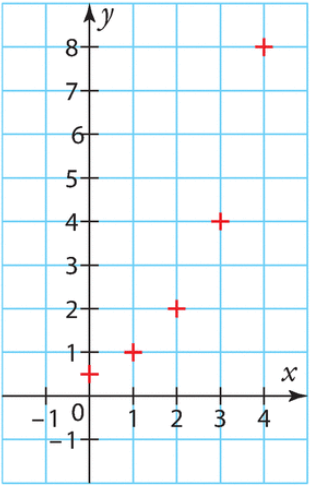
\includegraphics[scale=.6]{croissant.png}
    \end{center}
  \end{minipage}
  \hfill
  \begin{minipage}{.45\textwidth}
    Soit $u$ la suite géométrique de premier terme $u_0=5$ et de raison
    $r=\frac{1}{3}$.
    On a donc
    \[
      u_n = 5\times \frac{1}{3^n}.
    \]
    \begin{center}
      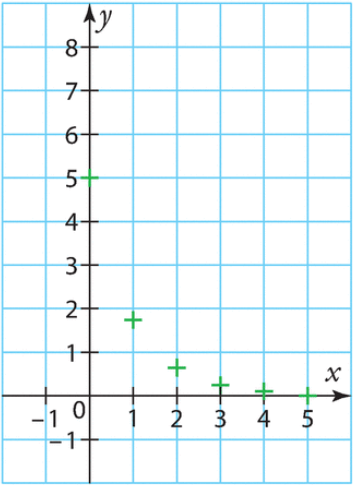
\includegraphics[scale=.6]{decroissant.png}
    \end{center}
  \end{minipage}
\end{exemple}

\subsection{Sens de variation}

\begin{prop}
  Soit $\left( u_n \right)$ une suite géométrique de raison $q$ dont les termes
  sont strictement positifs.
  \begin{itemize}
    \item Si $q>1$, alors la suite est strictement \textbf{croissante}.
    \item Si $q=1$, alors la suite est \textbf{constante}.
    \item Si $0<q<1$, alors la suite est \textbf{décroissante}.
  \end{itemize}
\end{prop}

\begin{rmq}
  Soit $\left( u_n \right)$ une suite géométrique de raison $q$.
  \begin{itemize}
    \item Si $q>0$ mais que les termes de la suite $(u_n)$ sont strictement
      négatifs, les sens de variations sont inversés par rapport à la propriété
      ci-dessus.
    \item Si $q=0$, la suite est presque toujours nulle, excepté éventuellement
      pour $u_0$.
    \item Si $q<0$, alors la suite n'est \textbf{pas monotone}.
  \end{itemize}
\end{rmq}

\subsection{Suite auxiliaire et suite arithmético-géométrique}
\begin{app}
  Un youtubeur compte $75$ abonnés le $1^\text{er}$ Janvier $2019$. Il remarque
  que, chaque mois, il en perd $40$\% et $100$ nouvelles personnes le suivent.
  On souhaite déterminer l'évolution de son nombre d'abonnés. On modélise la
  situation par une suite $\left( u_n \right)$, où $u_n$ est le nombre d'abonnés
  $n$ mois après Janvier $2019$.
  \begin{enumerate}
    \item Calculer le nombre d'abonnés au $1^\text{er}$ Février $2019$.
    \item Justifier que, pour tout entier $n\in\mathbb{N}$,
      $u_{n+1}=0,6u_n+100$.
    \item À l'aide de la calculatrice, déterminer le nombre de mois nécessaires
      pour dépasser les $230$ abonnés.
    \item Pour tout entier naturel $n\in\mathbb{N}$, on note $\left( v_n
      \right)$ la suite définie par $v_n = u_n-250$.
      \begin{enumerate}
        \item Exprimer $v_{n+1}$ en fonction de $v_n$. En déduire la nature de
          la suite $\left( v_n \right)$.
        \item Exprimer $v_n$ en fonction de $n$, puis $u_n$ en fonction de $n$.
        \item Déterminer le nombre d'abonnés au $1^\text{er}$ Décembre $2019$.
      \end{enumerate}
  \end{enumerate}
\end{app}

\section{Calculs de sommes}
\subsection{Propriétés générales}
\begin{notation}
  La \textbf{somme} des $n$ termes $x_1$, $x_2$, $\dots$, $x_n$ se note
  \[
    \sum_{k=1}^n x_k = x_1 + x_2 + \cdots + x_n.
  \]
\end{notation}
\begin{rmq}
  La lettre utilisée comme indice de sommation n'a pas d'importance : il s'agit
  d'une \textbf{variable «~muette~»}. On a donc
  \[
    \sum_{k=1}^n x_k =
    \sum_{i=1}^n x_i =
    \sum_{j=1}^n x_j
  \]
\end{rmq}
\begin{prop}
S'il n'y a pas d'indice de sommation dans la somme, c'est que le terme sommé
est constant.
  \[
    \sum_{k=1}^{n} 1 = \underbrace{1+1+\dots+1}_{n\text{ termes égaux à }1}
  \]
\end{prop}
\begin{app}
  Calculer les sommes suivantes.
  \begin{align*}
    \textbf{a)}\; & \sum_{k=1}^{15} 1 = &
    \textbf{b)}\; & \sum_{k=1}^{n} 1 = &
    \textbf{c)}\; & \sum_{k=0}^{15} 1 = &
    \textbf{d)}\; & \sum_{k=0}^{n} 1 =
  \end{align*}
\end{app}
\begin{prop}
  Soient $\left\{ x_k \right\}_{1\leq k \leq n}$ et $\left\{ y_k \right\}_{1\leq
  k \leq n}$ deux familles de $n$ nombres rééls et soit $\lambda\in\mathbb{R}$
  un réel. On a alors
  \begin{align*}
    \sum_{k=1}^n\left( x_k+y_k \right) &= \sum_{k=1}^nx_k+\sum_{k=1}^ny_k &
    &\text{et}&
    \sum_{k=1}^n\lambda x_k &= \lambda\sum_{k=1}^nx_k.
  \end{align*}
\end{prop}
\subsection{Somme des termes d'une suite arithmétique}
\begin{thm}
  Soit $n\in\mathbb{N}^*$ un entier naturel non nul, on a alors
  \[
    \sum_{k=1}^n k = 1+2+\cdots+n = \frac{n(n+1)}{2}.
  \]
\end{thm}
\begin{proof}[Démonstration (à connaître)]
  ~\vspace{3cm}\\
\end{proof}
\begin{app}
  Soit $n\in\mathbb{N}^*$. Calculer les sommes suivantes.
  \begin{align*}
    \textbf{a)}\;& \sum_{k=1}^{10} k &
    \textbf{b)}\;& \sum_{i=0}^{50} \left( 2i+1 \right) &
    \textbf{c)}\;& \sum_{k=0}^{n} (nk+3)
  \end{align*}

\end{app}
\subsection{Somme des termes d'une suite géométrique}

\end{document}
